\section{Дробові диференціальні рівняння}

Перш за все наведемо мінімальну мотивацію вивчення дробових диференціальних рівнянь. Нагадаємо, що класичне рівняння дифузії має вигляд
\begin{equation}
    \label{eq:classical-diffusion}
    \frac{\partial u}{\partial t} - k \sum_{i = 1}^n \frac{\partial^2 u}{\partial x_i^2} = f(x, t),
\end{equation}
де функція $f(x, t)$ відповідає джерелам речовини, що дифузує. \medskip

Втім, у реальному житті зустрічаються процеси, у яких дифузія відбувається повільніше/швидше, ніж передбачає рівняння \eqref{eq:classical-diffusion}. Для постановки відповідних рівнянь необхідно вводити дробові похідні (похідні дробових порядків).

\subsection{Основи дробового числення}

Розглянемо $f(t): \RR_{\ge 0} \to \RR$. Позначимо
\begin{equation}
    (I_0^1 f)(t) = \int_0^t f(s) \diff s.
\end{equation}
Також визначимо рекурсивно 
\begin{equation}
    (I_0^n f)(t) = I_0^1 (I_0^{n - 1} f)(t) = \int_0^t \int_0^{s_1} \cdots \int_0^{s_{n - 1}} f(s_n) \diff s_n \ldots \diff s_1.
\end{equation}

Подібне визначення не дуже зручне з обчислювальної точки зору, тому наступна теорема стане нам у пригоді.

\begin{theorem}[формула Коші-Діріхле]
    Для $f \in L_1([0, T])$, $t \in [0, T]$ має місце
    \begin{equation}
        (I_0^n f)(t) = \frac{1}{(n - 1)!} \int_0^t (t - s)^{n - 1} f(s) \diff s.
    \end{equation}
\end{theorem}
\begin{proof}
    Доведення проведемо за методом математичної індукції по $n$. \textbf{База} $n = 1$ виконується безпосередньо за визначенням $I_0^1$. \textbf{Перехід}: нехай
    \begin{equation}
        (I_0^n f)(t) = \frac{1}{(n - 1)!} \int_0^t (t - s)^{n - 1} f(s) \diff s.
    \end{equation}
    Тоді 
    \begin{equation}
        \begin{aligned}
            (I_0^{n + 1} f)(t) &= I_0^1 (I_0^n f)(t) = \int_0^t (I_0^n f)(s) \diff s = \\
            &= \int_0^t \frac{1}{(n - 1)!} \left( \int_0^s (s - \xi)^{n - 1} f(\xi) \diff \xi \right) \diff s = \\
            &= \frac{1}{(n - 1)!} \int_0^t \int_\xi^t f(\xi) (s - \xi)^{n - 1} \diff s \diff \xi = \\
            &= \frac{1}{(n - 1)!} \int_0^t f(\xi) \left. \frac{(s - \xi)^n}{n} \right|_{s = \xi}^{s = t} \diff \xi = \\
            &= \frac{1}{n!} \int_0^t f(\xi) (t - \xi)^n \diff \xi.
        \end{aligned}
    \end{equation}
    З точністю до назв змінних отримали що хотіли.
\end{proof}
\begin{remark}
    Перехід від другого рядка до третього тут відбувається за теоремою Фубіні. Наступна картинка може допомогти у розумінні:
    \begin{figure}[H]
        \centering
        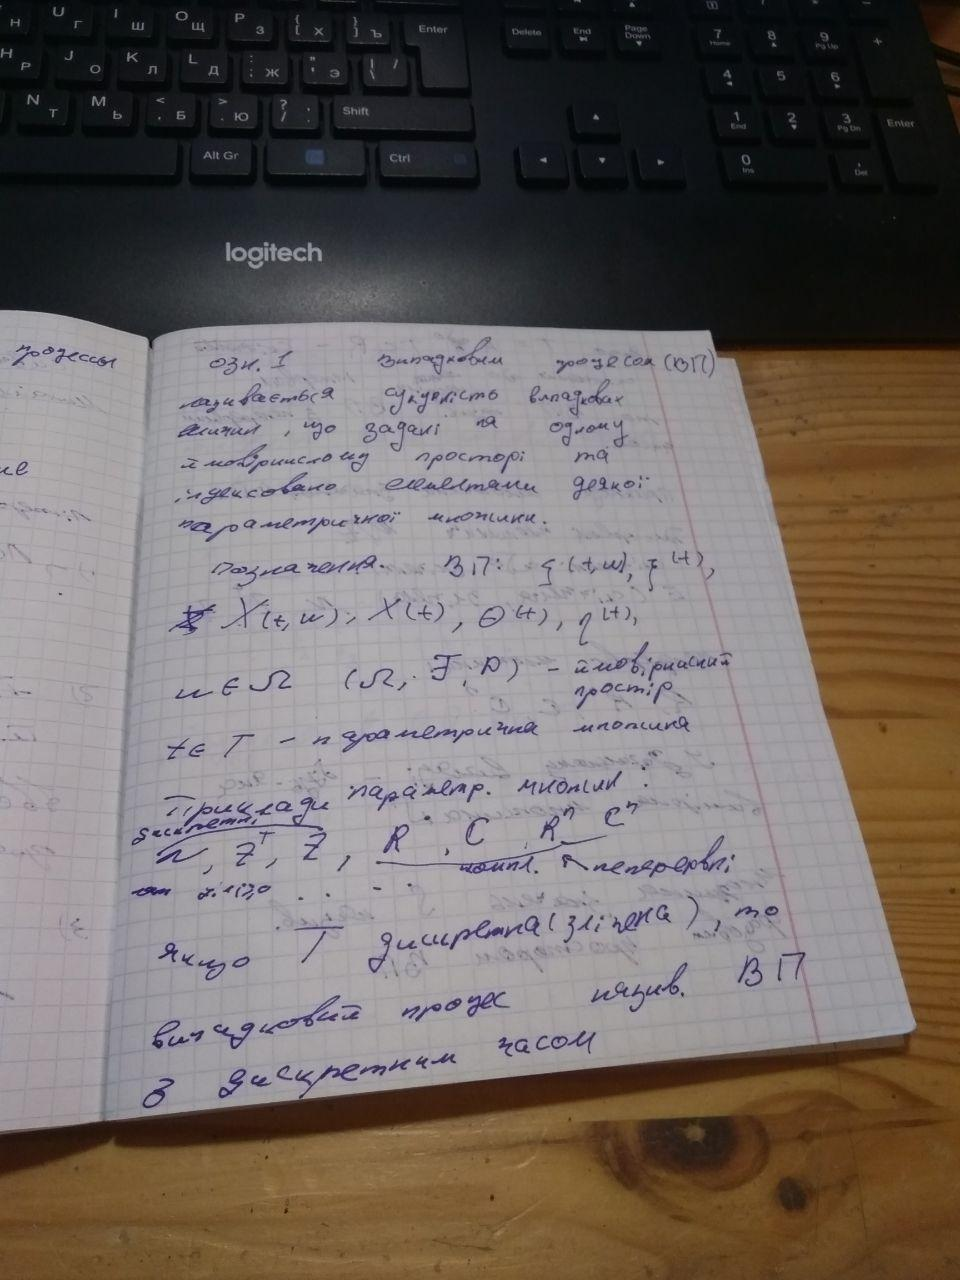
\includegraphics[width=.4\textwidth]{{img/01/01}.mps}
        \caption{При $s: 0 \to t$ маємо $\xi: 0 \to s$.}
    \end{figure}
\end{remark}

Формула Коші-Діріхле мотивує введення інтегральних операторів нецілого порядку.
\begin{definition}
    \textit{Інтегралом Рімана-Ліувілля} порядку $\alpha > 0$ з нижньою межею $0$ функції $f$ називається оператор
    \begin{equation}
        (I_0^\alpha f)(t) = \frac{1}{\Gamma(\alpha)} \int_0^t (t - s)^{\alpha - 1} f(s) \diff s.
    \end{equation}
    Також окремо зауважимо, що $I_0^0 f = f$.
\end{definition}
\begin{example}
    Справді, для $\alpha \in \NN$ маємо $\Gamma(\alpha) = (\alpha - 1)!$, тобто власне формулу Коші-Діріхле.
\end{example}
\begin{remark}
    Нагадаємо, що $\Gamma(\alpha) = \int_0^\infty e^{-t} t^{\alpha - 1} \diff t$.
\end{remark}

Взагалі кажучи, подібний вираз нагадує функцію згортки зі степеневою функцією порядку $\alpha$:
\begin{equation}
    I_0^\alpha f = f \star y_\alpha,
\end{equation}
де $y_\alpha(t) = \frac{1}{\Gamma(\alpha)} t^{\alpha - 1}$, а операція $\star: (\RR_{\ge 0} \to \RR) \times (\RR_{\ge 0} \to \RR) \to \RR$ визначається наступним чином:
\begin{equation}
    (f \star g) (t) = \int_0^t f(s) g(t - s) \diff s.
\end{equation}

Давайте тепер поміркуємо, як можна визначити диференціалний оператор дробового порядку, маючи відповідні інтегральні оператори. Взагалі кажучи, єдиної відповіді на це питання немає, як показує наступна картинка:
\begin{figure}[H]
    \centering
    
\includegraphics[width=.5\textwidth]{{img/01/02}.mps}
    \caption{Різні способи визначення диференціального оператора нецілого порядку}
\end{figure}

Введемо наступне допоміжне поняття для спрощення подальших позначень і формулювань:
\begin{definition}
    Нехай $\alpha \in \RR$. Тоді \textit{стеля} $\lceil \alpha \rceil$ --- найменше ціле число, що не менше за $\alpha$. Також інколи кажуть \textit{верхня ціла частина} $\alpha$.
\end{definition}

Нехай $\alpha > 0$, $n = \lceil \alpha \rceil$. 

\begin{definition}
    \textit{Похідною за Капуто} функції $f$ порядку $\alpha$ з нижнею межею $0$ називається оператор
    \begin{equation}
        ({}^\star D_0^\alpha f)(t) = I_0^{n - \alpha} \left( \frac{\diff^n f}{\diff t^n} \right).
    \end{equation}
\end{definition}
\begin{definition}
    \textit{Похідною Рімана-Ліувілля} функції $f$ порядку $\alpha$ з нижнею межею $0$ називається оператор
    \begin{equation}
        (D_0^\alpha f)(t) = \frac{\diff^n}{\diff t^n} \left( I_0^{n - \alpha} f \right).
    \end{equation}
\end{definition}

\begin{example}
    На рисунку вище $D_0^{0.5} = \dfrac{\diff}{\diff t} I_0^{0.5}$, а ${}^\star D_0^{0.5} = I_0^{0.5} \left( \dfrac{\diff}{\diff t} \right)$.
\end{example}

Взагалі кажучи виникає питання коли введені вище похідні існують. Для відповіді на це питання нам знадобиться наступне:
\begin{definition}
    Функція $f$ називається \textit{абсолютно неперервною} (\textit{eng.} AC, absolutely continuous) на проміжку $I$ якщо $\forall \epsilon > 0$: $\exists \delta > 0$: $\forall x_1 < y_1 \le x_2 < y_2 \le \ldots \le x_n < y_n$: 
    \begin{equation}
        \sum_{k = 1}^n (y_k - x_k) < \delta \implies \sum_{k = 1}^n |f(y_k) - f(x_k)| < \epsilon.
    \end{equation}
\end{definition}

Так от для AC функцій їхні похідні інтегровні (з нецілим порядком), тобто похідні (з нецілим порядком) існують. \medskip

Поняття абсолютної неперервності має нагадувати поняття рівномірної неперервності (\textit{eng.} UC, uniformly continuous). Зрозуміло, що з абсолютної неперервності випливає ($n = 1$) рівномірна неперервність, але зворотнє не виконується. 

\begin{exercise}
    Наведіть приклад рівномірно неперервної але не абсолютно неперервної функції.
\end{exercise}
\begin{solution}
    Функція Кантора є класичним прикладом такої функції. нагадаємо, що функція Кантора визначається як
    \begin{equation}
        c(x) = \begin{cases}
            \frac{1}{2} \Sum_{n = 1}^\infty \frac{b_n}{2^n}, & x = \Sum_{n = 1}^\infty \frac{b_n}{3^n} \in \mathcal{C}, \\
            \Sup_{y \le x, y \in \mathcal{C}} c(y), & x \in [0, 1] \setminus \mathcal{C},
        \end{cases}
    \end{equation}
    де $\mathcal{C}$ --- множина Кантора, а $b_n$ --- тернарні ``біти'' числа $x$, тобто $b_n \in \{0, 2\}$. \medskip
    
    Для наглядності наведемо графік функції Кантора:
    \begin{figure}[H]
        \centering
        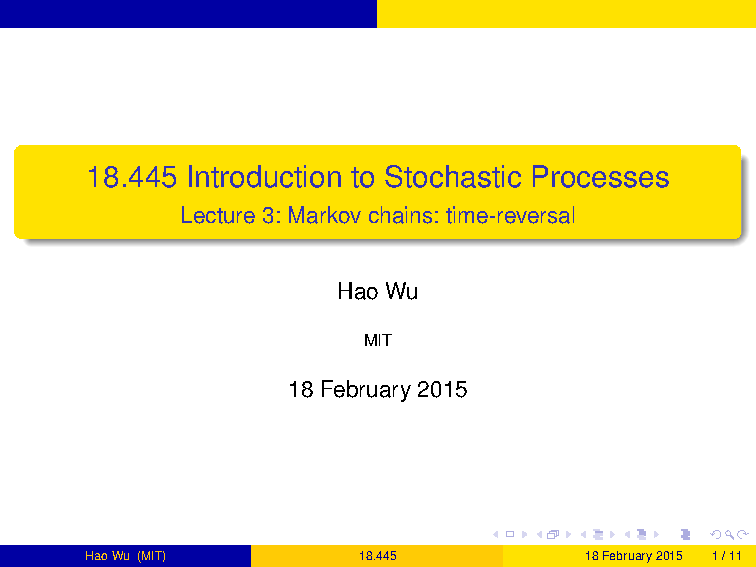
\includegraphics[width=.5\textwidth]{{img/01/03}.png}
        \caption{функція Кантора}
    \end{figure}
    
    Як і кожна неперервна функція на компакті ($[0,1]$), вона є рівномірно неперервною на ньому. Втім, вона не є абсолютно неперервною, адже $\mu(\mathcal{C}) = 0$, тобто $\forall \delta > 0$ знайдуться інтервали сумарною довжиною $<\delta$ що покривають $\mathcal{C}$, а тому зміна значення $c(\cdot)$ на них складатиме $1 > \epsilon$.
\end{solution}

Виникає закономірне запитання: чи існує аналог формули Коші-Діріхле для диференціальних операторів? Виявляється, що так, хоча він і не зовсім такий, як можна було б очікувати.

\begin{theorem}
    Нехай $f \in AC^n([0, T])$, $t \in [0, T]$, $n = \lceil \alpha \rceil$. Тоді
    \begin{equation}
        (D_0^\alpha f) (t) = \frac{1}{\Gamma(n - \alpha)} \int_0^t \frac{f^{(n)}(s)}{(t - s)^{\alpha + 1 - n}} \diff s + \sum_{k = 0}^{n - 1} \frac{f^{(k)}(0)}{\Gamma(1 + k - \alpha) t^{\alpha - k}}.
    \end{equation}
\end{theorem}
\begin{example}
    Зокрема, при $0 < \alpha < 1$ маємо $f \in AC([0, T])$ і
    \begin{equation}
        (D_0^\alpha f) (t) = \frac{1}{\Gamma(1 - \alpha)} \int_0^t \frac{f'(s)}{(t - s)^\alpha} \diff s + \frac{f(0)}{\Gamma(1 - \alpha) t^\alpha}.
    \end{equation}
\end{example}
\begin{remark}
    Як показує формула, ${}^\star D_0^\alpha, D_0^\alpha$ --- нелокальні оператори.    
\end{remark}
\begin{proof}
    Доведемо частинний випадок $0 < \alpha < 1$:
    \begin{equation}
        \begin{aligned}
            (D_0^\alpha f)(t) &= \frac{\diff}{\diff t} I_0^{1 - \alpha} f = \frac{\diff}{\diff t} \frac{1}{\Gamma(1 - \alpha)} \int_0^t (t - s)^{-\alpha} f(s) \diff s = \\
            &= \frac{\diff}{\diff t} \frac{1}{\Gamma(1 - \alpha)} \int_0^t f(s) \frac{\diff (-(t-s)^{1-\alpha}}{1 - \alpha} \diff s = \\
            &= \frac{\diff}{\diff t} \frac{1}{\Gamma(1 - \alpha)} \left( \left. \frac{-f(s)(t-s)^{1-\alpha}}{1 - \alpha} \right|_{s = 0}^{s = t} + \int_0^t f'(s) \frac{(t - s)^{1- \alpha}}{1 - \alpha} \diff s \right) = \\
            &= \frac{\diff}{\diff t} \frac{1}{\Gamma(1 - \alpha)} \left( \frac{f(0) t^{1-\alpha}}{1 - \alpha} + \frac{1}{1 - \alpha} \int_0^t f'(s) (t - s)^{1 - \alpha} \diff s \right) = \\
            &= \frac{1}{\Gamma(1 - \alpha)} \left( \frac{f(0)}{t^\alpha} + \int_0^t f'(s) (t - s)^{- \alpha} \diff s \right).
        \end{aligned}
    \end{equation}
\end{proof}
\begin{remark}
    Тут при переході від другого рядочка до третього ми скористалися інтегруванням за частинами, а в останньому переході --- формулою Лейбніца:
    \begin{equation}
        \frac{\diff}{\diff x} \left(\int_{a(x)}^{b(x)} f(x,t) \diff t \right) = f(x, b(x)) \cdot b'(x) - f(x, a(x)) \cdot a'(x) + \int_{a(x)}^{b(x)} \frac{\partial}{\partial x} f(x,t) \diff t.    
    \end{equation}
\end{remark}

На завершення визначимо ще кілька корисних для подальшого дослідження об'єктів:
\begin{definition}
    \textit{Інтегралом Рімана-Ліувілля з нижньою }(\textit{лівою})\textit{ межею} $a$ називається
    \begin{equation}
        (I_{a^+}^\alpha f)(t) = \frac{1}{\Gamma(\alpha)} \int_a^t f(s) (t - s)^{\alpha - 1} \diff s.
    \end{equation}
\end{definition}
\begin{definition}
    \textit{Інтегралом Рімана-Ліувілля з правою }(\textit{верхньою})\textit{ межею} $T$ для $t < T$ називається
    \begin{equation}
        (I_{T^-}^\alpha f)(t) = -\frac{1}{\Gamma(\alpha)} \int_t^T f(s) (t - s)^\alpha \diff s.
    \end{equation}
\end{definition}
